\documentclass[12pt]{article}
\usepackage[utf8]{inputenc}
\usepackage{hyperref}
\usepackage{graphicx}
\usepackage{tikz}
\usetikzlibrary{patterns, arrows.meta, positioning}

\title{A Brief Introduction to the C Programming Language}
\author{Shaan Fulton}
\date{\today}

\begin{document}

\maketitle

C is a low-level high-level language. That is, it is ultimately a high level language, not an assembly language. We don't need to know exactly how the CPU and memory works. However, comapred with Java and Python, there is a lot less abstraction, especially around memory management.

We can think of Python as a modern electric vehicle. It's really hard to mess things up. The drivetrain is entirely abstracted.

\begin{figure}[htbp]
    \centering
    \includegraphics[width=0.7\textwidth]{python.png}
    \caption{Python as a car}
    \label{fig:python}
\end{figure}

With Java there is more to mess up. We have to manage types and can't have these imaginary arrays that grow in size magically, at least not out of the box. The drivetrain is largely abstracted, but we have to shift gears and start the car.

\begin{figure}[htbp]
    \centering
    \includegraphics[width=0.7\textwidth]{java.png}
    \caption{Java as a car}
    \label{fig:java}
\end{figure}

Then there's C. With C we don't get a gear shifter. We have to manually stick our hand into the transmission, pull on the clutch, and use our pinky fingers to align the synchronizer for every successful gear shift. It's very easy to lose a finger, or break your transmission, with C.

\begin{figure}[htbp]
    \centering
    \includegraphics[width=0.7\textwidth]{c.png}
    \caption{Good luck}
    \label{fig:c}
\end{figure}

\newpage

\section*{Compiling C}

All computers run on \textbf{machine code}: raw 1s and 0s that represent instructions for the CPU. These binary instructions can be written in a human-readable form called \textbf{assembly language}. For RISC-V, machine code is the binary encoding, and RISC-V assembly is the readable version of the same instructions.

\begin{center}
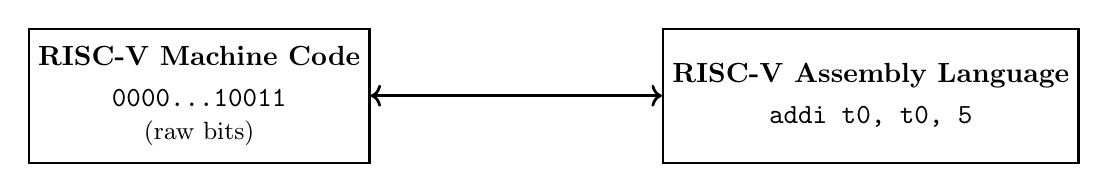
\begin{tikzpicture}[thick, node distance=3.7cm]
  % First box: RISC-V Machine Code
  \node[draw, rectangle, minimum width=3.3cm, minimum height=1.7cm, align=center] (machine) {
    \textbf{RISC-V Machine Code}\\[0.1cm]
    \texttt{0000\ldots10011}\\
    \small (raw bits)
  };
  % Second box: RISC-V Assembly Language
  \node[draw, rectangle, minimum width=3.3cm, minimum height=1.7cm, right=of machine, align=center] (assembly) {
    \textbf{RISC-V Assembly Language}\\[0.1cm]
    \texttt{addi t0, t0, 5}
  };
  % Arrow
  \draw[<->, line width=1pt] (machine) -- (assembly);
\end{tikzpicture}
\end{center}

Different machines use different machine code. x86, ARM, etc. — it's all different. We want C to run on all machines. To accomplish this, we must build a C compiler for every machine architecture that takes our C instruction set and converts it to the standard machine code instructions that a particular machine knows how to work with.

\begin{center}
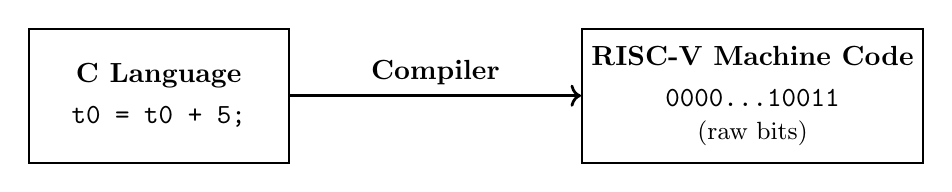
\begin{tikzpicture}[thick, node distance=3.7cm]
  % First box: C Language
  \node[draw, rectangle, minimum width=3.3cm, minimum height=1.7cm, align=center] (c) {
    \textbf{C Language}\\[0.1cm]
    \ttfamily t0 = t0 + 5;
  };
  % Second box: Machine Code
  \node[draw, rectangle, minimum width=3.3cm, minimum height=1.7cm, right=of c, align=center] (machine) {
    \textbf{RISC-V Machine Code}\\[0.1cm]
    \texttt{0000\ldots10011}\\
    \small (raw bits)
  };
  % Arrow with label
  \draw[->, line width=1pt] (c) -- node[above]{\textbf{Compiler}} (machine);
\end{tikzpicture}
\end{center}

And that is effectively all that the C compiler does, but there's a bit more nuance to it. Suppose we have multiple C files and we want to tie them all together. Maybe we want to add a library for math operations in, or we just have a large application with multiple files. The brute force compilation approach would require us to feed all of these files into our compiler and convert them to machine code for even a small change to one file. That's an excessive amount of compilation.

Instead, we actually compile \textbf{(or assemble)} each file seperately into machine code that lacks essential headers and linking to other files. \textbf{These are .o files}. Whenever we make a change, we just update the relevant .o machine code file. Then, when we're ready to run our app, we run a linker that combines all these .o machine code files together and outputs a single .out machine code executable file with headers and all.

\begin{figure}
\centering
\begin{tikzpicture}[
  node distance=1.2cm and 1.2cm,
  every node/.style={font=\sffamily\small},
  file/.style={draw, rectangle, minimum width=1.4cm, minimum height=0.8cm},
  process/.style={
    draw,
    rectangle,
    pattern=north east lines,
    pattern color=gray,
    minimum width=1.4cm,
    minimum height=0.8cm
  },
  lib/.style={draw, ellipse, minimum width=1.6cm, minimum height=0.8cm},
  arrow/.style={-Latex}
]

% Nodes
\node[file] (source1) {Source file};
\node[process, right=of source1] (asm1) {Assembler};
\node[file, right=of asm1] (obj1) {Object file};

\node[file, below=of source1] (source2) {Source file};
\node[process, right=of source2] (asm2) {Assembler};
\node[file, right=of asm2] (obj2) {Object file};

\node[file, below=of source2] (source3) {Source file};
\node[process, right=of source3] (asm3) {Assembler};
\node[file, right=of asm3] (obj3) {Object file};

\node[process, right=1.6cm of obj2] (linker) {Linker};
\node[file, right=of linker] (exe) {Executable file};
\node[lib, below=of linker] (lib) {Program library};

% Arrows
\draw[arrow] (source1) -- (asm1);
\draw[arrow] (asm1) -- (obj1);
\draw[arrow] (source2) -- (asm2);
\draw[arrow] (asm2) -- (obj2);
\draw[arrow] (source3) -- (asm3);
\draw[arrow] (asm3) -- (obj3);

\draw[arrow] (obj1) -- (linker);
\draw[arrow] (obj2) -- (linker);
\draw[arrow] (obj3) -- (linker);
\draw[arrow] (lib) -- (linker);
\draw[arrow] (linker) -- (exe);

\end{tikzpicture}
\caption{Assembly and linking process from multiple source files}
\label{fig:assembly-linking}
\end{figure}

\subsection*{How C Compilation is Different}

Not all languages compile this way.

For example, Python is an interpreted language. When you run a Python script, the source code is directly executed by the Python interpreter, line by line. There is no separate compilation step producing an executable file in advance.

Java, on the other hand, compiles source code into an intermediate form called bytecode. This bytecode is not executed directly by the operating system but runs inside the Java Virtual Machine (JVM), which interprets or just-in-time compiles it at runtime.

The advantage of these systems is that these virtual environments or interpreters can be made extremely robust so that they work the exact same way on every machine. With C code, because we're directly compiling it, there's actually quite a number of differences in how different machines assemble our code. For instance, in some machines integers are 16-bits, whereas in others they are 32-bits. C doesn't care that this causes extreme incompatibility issues. That's just C for you.

\subsection*{The C Pre-Processor}

Just one more detail here. Before C is sent off to be assembled, the C pre-processor tacks additional C code into our C file. The C pre-processor (CPP) is actually quite useful. It's like a little script that runs through your code and looks for little `\#' symbols. When it finds one it does as it is commanded: adding in a header, macro, or whatever. For instance, we can create a macro (mini standardized function) like:

\begin{verbatim}
#define min(x,y) ((x) < (y) ? (x):(y))
\end{verbatim}

Now, wherever we write our little min function throughout our C file, the C pre-processor will replace it with code that is actually useful.

\end{document}

